% vim:set et sw=2 ts=4 tw=72:
\chapter{Background}\label{chap:background}

To understand how a change is integrated into the master branch of a
repository, it is vital to understand the merges that led to the
integration of the commit, and the commits that are merged into the
master branch with the commit of interest. Maintainers of software must
sift through the commits to determine which changes being made to the
current version of the software pertain to the area of the software that
they are maintaining. Specifically, maintainers must be able to answer
two questions;

\begin{textbox}
\begin{itemize}
  \item How is a commit integrated?
  \item What other commits are related to a given commit?
\end{itemize}
\end{textbox}

Commits being integrated into a repository may pass through multiple
merges on the path to the master branch. The merges form logical
groupings of related code; furthermore, in some repository structures,
merges are used to resolve conflicts between commits. In order to apply
the changes in one commit, modifications to other parts of the codebase
may be necessary. While they are necessary to the integration of the
commit of interest, these modifications will likely be in separate
commits, and possibly merged into the branch that the commit of interest
is on. Maintainers must be able to easily find these commits, as they
will be necessary for back-porting the commit of interest into older
versions of the software.

We specifically study the Linux kernel repository. Older versions of the
Linux kernel are used in a wide variety of situations including various
Linux desktop distributions, internet of things device firmware, web
servers, spacecrafts\footnote{Linux is used heavily at SpaceX
  \url{https://lwn.net/Articles/540368/}}, and in mobile devices as the
base of the Android platform. These kernels are sometimes modified forks
of the official Linux kernel, made to be more suitable for the specific
needs of the application. Due to these application-specific
modifications, it is not feasible to update to the latest version of the
kernel for every official update. While it may not be feasible to
update, the changes being made to the official version are necessary as
they fix bugs, patch security issues, and improve performance. Due to
the sometimes critical nature of the patches being merged into the
current version of the kernel, it is necessary for maintainers working
on application-specific forks of the kernel to sift through the commits
coming into the official version, looking for the changes that may
impact the kernel they are maintaining. In Section~\ref{sec:linux}, we
describe the structure of the Linux repository, the dataset collected
from the repository, and investigate the nature of the repository
integration and merge behaviour.

Linux uses git as the version control system, managing the distributed
nature of the kernel development and storing the changes to the kernel.
In Section~\ref{sec:git}, we discuss the structure of git, repository
visualizations available, and challenges it poses against answering the
two main questions.

\section{Linux}\label{sec:linux}

Linux is open source, using git to track and manage the source code in
the kernel. A mirror of the repository is available on
GitHub\footnote{\url{https://github.com/torvalds/linux}}, which makes
data collection relatively straightforward. In this section, we describe
the dataset that we collected, looking at the number of authors,
commits, and merges.

The data extracted from the repository involves all merges into the
master branch between April 18, 2005 and August 14, 2014. This
corresponds to the merges added to the kernel between versions 2.6.11
and Linux 3.16. The commits collected from the repository include
commits authored between September 17, 2001 and December 6, 2014. There
are 4 commits in the dataset that are beyond this range due to the date
being incorrectly set on that developer's machine. There is one
incorrect date that is dated January 1, 1970, authored by Ursula Braun,
and three commits dated after 2014. These commits are dated April 5,
2019, October 14 2030, and April 25 2037, authored by Len Brown, Yanmin
Zhang, and Daniel Vetter, respectively. Commits are not necessarily
merged immediately, all commits were added between April 15, 2005 and
October 14, 2014. The average difference between when a commit was
created and when it was committed is 16 days and 10 hours; 25\% of the
commits were committed within 2 hours of being authored, 50\% committed
within 2 days and 8 hours, 75\% within 15 days, and all commits were
merged within 9.5 years of being authored. In this breakdown of the
kernel data, we will focus on the commits integrated into kernel
versions Linux 3.1 to Linux 3.16, translating to the merges between July
21, 2011 and August 3, 2014.

\evan{How much of this should I be describing here versus in in a later
section?}

As expected, we find that the Linux kernel is highly collaborative, and
is very active. Between 1000 and 1500 authors have contributions
accepted into the official kernel per release (shown in
Figure~\ref{fig:linux_authors_per_release}). These authors contribute
between 8000 and 14000 commits per release
(Figure~\ref{fig:linux_commits_per_release}). Between 275 and 400 merges
integrate the commits into the master branch of the kernel per release
(Figure~\ref{fig:linux_commits_per_release}). The Linux kernel
repository is a prime example of a successful open source project,
exemplifying the collaborative nature of modern software development.
The sheer number of commits being contributed make the task of filtering
the important or relevant commits impractical.

\evan{Having some troubles getting enough text mixed in with the plots.
  Should I just move some of them to the appendix later?}

\begin{figure}[htpb]
  \centering
  \includegraphics[width=0.8\linewidth]{Figures/background/linux_authors_per_release.pdf}
  \caption{Unique authors with contributions to each kernel version}
  \label{fig:linux_authors_per_release}
\end{figure}

\begin{figure}[htpb]
  \centering
  \includegraphics[width=0.8\linewidth, page=1]{Figures/background/linux_commits_per_release.pdf}
  \caption{Commits per release from Linux 3.1 to Linux 3.16}
  \label{fig:linux_commits_per_release}
\end{figure}

\begin{figure}[htpb]
  \centering
  \includegraphics[width=0.8\linewidth, page=2]{Figures/background/linux_commits_per_release.pdf}
  \caption{Merges per release from Linux 3.1 to Linux 3.16}
  \label{fig:linux_merges_per_release}
\end{figure}

While the number of integrating merges into the master branch appears to
be decreasing slightly per release, the number of commits per release is
increasing. The average (mean) number of commits per merge per release
has increased from slightly over 20 commits per merge in Linux 3.1 up to
50 commits per merge in Linux 3.16
(Figure~\ref{fig:linux_commits_per_merge_per_release}).

\begin{figure}[htpb]
  \centering
  \includegraphics[width=0.8\linewidth, page=3]{Figures/background/linux_commits_per_release.pdf}
  \caption{Commits per merge into each release of Linux from 3.1 to 3.16
    \evan{Should probably go in the appendix}}
  \label{fig:linux_commits_per_merge_per_release}
\end{figure}

Grouping commits by the merge that integrates it into the master branch,
we get a different view of the kernel. The individual merges contain
relatively few commits, 25\% of the merges merge only a single commit,
and 50\% of the merges merge at most 7 events
(Figure~\ref{fig:linux_merge_distribution_per_release}).

\begin{figure}[htpb]
  \centering
  \includegraphics[width=0.8\linewidth]{Figures/background/linux_merge_distribution_per_release.pdf}
  \caption{Distribution of Merge Sizes per Release Between Linux 3.1 and
  3.16}
  \label{fig:linux_merge_distribution_per_release}
\end{figure}

Initially, the repository looks very large and unmanageable. Breaking
the commits down by the integrating merge looks like a promising means
of simplifying the content. Most of the groups of commits will only
contain 7 elements, which is nearly trivial to visualize.

\section{Git}\label{sec:git}

\define{Version control software}{VCS} supports software development,
assisting with efficient storage of code, archival of the modifications,
and navigation of code. The goals of version control software is to
provide means of efficient source code storage, logging changes made to
the code, and retrieving historical versions. Source Code Control System
(SCCS) and its successor, Revision Control System (RCS), were designed
for local development, providing no means of collaboration. As software
projects grew, this model quickly became outdated, being replaced by a
client-server model. \define{Concurrent Versions System}{CVS} and Apache
\define{Subversion}{SVN} are examples of two client-server VCSs, which
adds support for collaborative development. As projects grew, the
client-server was no longer sufficient to meet the requirements of
development teams, which gave rise to the \define{distributed version
  control system}{DVCS}. Distributed version control systems are more
flexible than either the local systems or client-server systems as they
give the user more control of their local clone and have further support
for distributed workflows. The distributed version control is necessary
for large open source projects, like Linux, it does pose additional
challenges related to the complexities that arise as a result of being
distributed.

Git is a DVCS, implemented for handling development on the Linux kernel,
written to replace BitKeeper due to issues with highly restrictive
licensing in April of 2005. The primary goals for git were to be able to
support development of the kernel, be implemented quickly so as not to
hinder the development of the kernel, and to maintain similar levels of
patch granularity as BitKeeper\footnote{initial announcement of git on
  the mailing list
  \url{https://marc.info/?l=linux-kernel&m=111280216717070}}. The
initial version of git was around 1300 lines of code and was written and
self-hosting in less than 2 weeks\footnote{From the git mailing list
  \url{https://marc.info/?l=git&m=117254154130732}}.

The core model used to store the repository is a \define{directed
  acyclic graph}{DAG}. Git refers to the nodes of the DAG as commits,
not distinguishing between the code-carrying commits and the structural
commits that merge two branches together. In this \paper{}, we will
refer to the code-carrying commits as commits, the structural merge
commits as merges, and refer to both types without discrimination as
repository events. Each repository event contains an ordered list of one
or more parents, except the initial commit which has no parents. The
parent relationship points from the current event toward the initial
commit. Commits have a single parent, while merges will have at least
two parents, the parent on the current branch followed by the repository
events being merged. This model allows merging of multiple branches
simultaneously in octopus merges, where the order of the parents
represents the order that the branches were specified for being
merged\footnote{One octopus merge in Linux
  (2cde51fbd0f310c8a2c5f977e665c0ac3945b46d) has 66 parents}.
A \foxtrot\footnote{See
  \url{http://bit-booster.blogspot.ca/2016/02/no-foxtrots-allowed.html}
  for a full description of the issue.} merge occurs when the parent on
the current branch is replaced by a parent from a branch being merged
into the current branch, thus confounding the branch relationships
(depicted in Figure~\ref{fig:foxtrot_steps}).

\begin{figure}[htpb]
  \centering
  \begin{tabular}{ccc}
    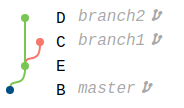
\includegraphics[width=114px]{Figures/background/foxtrot_initial.png} &
    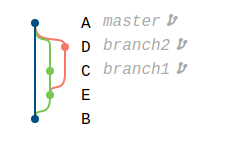
\includegraphics[width=145px]{Figures/background/foxtrot_good.png} &
    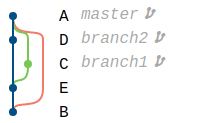
\includegraphics[width=145px]{Figures/background/foxtrot_bad.png} \\
    Initial Repository & No Foxtrot & Foxtrot
  \end{tabular}
  \caption{Depiction of a foxtrot merge, where the master branch is
    confounded by \emph{branch2}}
  \label{fig:foxtrot_steps}
\end{figure}

The repository events in the DAG are immutable; once a repository event
is created, it can't be changed. Git allows operations to alter
repository events and re-order them, but this will create a new event
with a new commit hash. This property makes a repository event unable to
record the traversal of merges into the master branch of the repository.
Introducing an additional field to track the path to the master branch
would create a circular dependency between the parent and child. Any
updates to the DAG would modify the commit hashes for all repository
events in the repository. To alleviate this, git provides the command
\verb|git log --children| which traverses the DAG and prints the
inverted edges relationship between events.

Under perfect conditions, visualizations of the DAG should show how a
commit is integrated as the DAG stores all information about the
repository, and the events within. It includes information about where
branches are being made, where merges are occurring, who is making
changes, when the changes are being made, what files are being modified,
and how much is being changed. Most repositories are simple, with only a
few small branches and a clear well-defined master branch; however, in
large, active, repositories, the master branch can be confounded by
\foxtrot{} merges, making it difficult to identify. This consequently
would make it difficult to determine how a commit is merged.
